\documentclass[12pt,a4paper]{article}

\usepackage[a4paper, margin=2.5cm]{geometry}
\usepackage{amsmath, amssymb}
\usepackage{graphicx}
\usepackage{booktabs}
\usepackage{hyperref}
\usepackage{caption}
\usepackage{subcaption}
\usepackage{enumitem}
\usepackage{setspace}
\usepackage{parskip}

\onehalfspacing

\title{\textbf{Reliability Assessment of the JAXA H3 Fairing under Manufacturing Variability\\
Using Polynomial Chaos Expansion as a Stochastic FEM Surrogate}}

\author{Keisuke Nishioka\\
Matriculation Number: 10081049\\[0.5em]
Supervisor: Dr.\ Zhibao Zheng\\
Examiner: Prof.\ Dr.-Ing.\ Udo Nackenhorst\\[0.5em]
Institut f\"{u}r Baumechanik und Numerische Mechanik\\
Leibniz Universit\"{a}t Hannover}

\date{May 2026}

\begin{document}

\maketitle
\newpage

\tableofcontents
\newpage

\listoffigures
\listoftables
\newpage

%------------------------------------------------------------------
\section{Abstract}
%------------------------------------------------------------------

This study applies non-intrusive Polynomial Chaos Expansion (PCE) with Smolyak sparse quadrature as a Stochastic Finite Element Method (SFEM) surrogate to quantify how manufacturing variability in five key material parameters propagates to structural responses in the JAXA H3 rocket fairing. The fairing is a Carbon Fiber Reinforced Polymer (CFRP)/aluminum-honeycomb sandwich structure modelled in Abaqus/Standard. Five independent truncated-normal uncertain parameters are considered: fiber-direction modulus $E_1$, in-plane shear modulus $G_{12}$, cohesive zone stiffness $K_n$, Mode-I fracture energy $G_{Ic}$, and cohesive strength $t_n$.

PCE at degree 2 (66 Abaqus simulations via Smolyak sparse grid) achieves full convergence; degree 3 (286 simulations) yields identical statistics. Global sensitivity analysis via Sobol indices reveals that $E_1$ accounts for over 99\% of output variance in both peak von Mises stress and maximum displacement. The peak stress mean is 209.7~MPa with a coefficient of variation of 1.13\%, well below the 1{,}200~MPa CFRP failure threshold, yielding zero failure probability. The cohesive zone never activates under the design load. A neural network (MLP) surrogate trained on the same data is used for comparison; PCE achieves equal or better accuracy with full analytical interpretability.

\textbf{Keywords:} Polynomial Chaos Expansion, Stochastic Finite Element Method, Sobol sensitivity indices, reliability analysis, CFRP, composite structures, JAXA H3

%------------------------------------------------------------------
\section{Literature Review}
%------------------------------------------------------------------

The quantification of uncertainty arising from manufacturing variability in composite aerospace structures is a fundamental challenge in structural reliability engineering. Stochastic Finite Element Methods (SFEM) provide a rigorous framework to propagate input uncertainties through deterministic computational models.

Ghanem and Spanos~\cite{ghanem1991} introduced the spectral approach to SFEM, representing stochastic processes via Polynomial Chaos Expansion (PCE). In their formulation, uncertain system responses are expanded in a series of Hermite polynomial basis functions of standard Gaussian random variables, enabling the transformation of stochastic boundary-value problems into systems of deterministic equations. This intrusive approach forms the theoretical foundation of PCE-based SFEM.

Sudret and Der Kiureghian~\cite{sudret2000} provided a comprehensive state-of-the-art review of SFEM and reliability analysis, comparing intrusive spectral methods with non-intrusive sampling-based approaches. Non-intrusive PCE, in which the existing deterministic FEM code is treated as a black-box and PCE coefficients are estimated via regression or quadrature, substantially reduces implementation effort. Sudret~\cite{sudret2008} further demonstrated that once a PCE surrogate is constructed, global sensitivity indices in the sense of Sobol can be obtained analytically at negligible additional cost, making PCE particularly attractive for combined uncertainty quantification and sensitivity analysis.

Smolyak sparse quadrature~\cite{smolyak1963} addresses the curse of dimensionality inherent in full tensor-product Gauss quadrature. For $d$ uncertain parameters and polynomial degree $p$, Smolyak grids achieve the same exactness as full grids while reducing the number of function evaluations from $\mathcal{O}(n_q^d)$ to $\mathcal{O}(n_q (\log n_q)^{d-1})$. Fajraoui et al.~\cite{fajraoui2017} extended sparse PCE to sequential experimental designs, further improving efficiency for high-dimensional problems.

Global sensitivity analysis through Sobol indices~\cite{saltelli2008} decomposes the total output variance into contributions from individual inputs and their interactions. First-order indices $S_i$ quantify the variance reduction achieved by fixing input $X_i$; total-order indices $S_T^i$ capture the full effect of $X_i$ including all interactions. In thin-walled composite structures, where deformation is predominantly governed by membrane stiffness, it is expected that fiber-direction modulus uncertainty dominates the structural response variance, as confirmed in this work.

%------------------------------------------------------------------
\section{Introduction}
%------------------------------------------------------------------

Composite fairing structures for launch vehicles, such as the JAXA H3 rocket, are manufactured from CFRP skins bonded to aluminum honeycomb cores. Material properties of CFRP and the adhesive cohesive zone are inherently variable due to manufacturing processes: fiber volume fraction fluctuations, cure cycle variations, and adhesive film thickness inconsistencies. These uncertainties propagate into structural responses---stress, damage, and deformation---affecting reliability.

This study applies \textbf{non-intrusive Polynomial Chaos Expansion (PCE)} as a Stochastic FEM surrogate to quantify how manufacturing variability in five key parameters propagates to structural responses in the H3 fairing. The existing high-fidelity Abaqus/Standard FEM model of the H3 fairing panel serves as the black-box FEM solver. A neural network (NN) surrogate trained on the same data provides a basis for comparison. The specific objectives are:

\begin{enumerate}
    \item Construct PCE surrogates of degree 2 and 3 using Smolyak sparse quadrature and validate convergence.
    \item Identify the dominant uncertain parameter via Sobol global sensitivity analysis.
    \item Assess structural reliability ($P_f$, $\beta$) under manufacturing variability.
    \item Compare PCE and NN surrogate accuracy and interpretability.
\end{enumerate}

%------------------------------------------------------------------
\section{Methodology}
%------------------------------------------------------------------

\subsection{Polynomial Chaos Expansion}

For a model response $Y = \mathcal{M}(\xi)$ depending on random input vector $\xi \in \mathbb{R}^d$, PCE approximates:
\begin{equation}
    Y \approx \hat{Y} = \sum_{\alpha \in \mathcal{A}} c_\alpha \Psi_\alpha(\xi)
\end{equation}
where $\Psi_\alpha$ are orthogonal polynomial basis functions (Hermite polynomials for Gaussian inputs), $c_\alpha$ are coefficients to be determined, and $\mathcal{A}$ is a truncated multi-index set with $|\alpha| \leq p$ (total degree $p$). For $d = 5$ variables and degree $p$, the number of basis terms is:
\begin{equation}
    P = \binom{d+p}{p} = \binom{5+p}{p}
\end{equation}
giving $P = 21$ for $p=2$ and $P = 56$ for $p=3$.

The choice of a Hermite basis is dictated by the Gaussian input measure rather than being arbitrary: Hermite polynomials are orthogonal with respect to the standard-normal weight, and it is this orthogonality, not the polynomial form itself, that makes the expansion valuable. Because the basis is orthogonal, the coefficients $c_\alpha$ coincide with the spectral projections of the response, so the mean is read directly from $c_0$ and the variance from the sum of the remaining squared coefficients, $\sum_{\alpha \neq 0} c_\alpha^2\,\mathbb{E}[\Psi_\alpha^2]$. The Sobol indices follow by the same mechanism, as partial sums of these squared coefficients grouped according to the variables each multi-index $\alpha$ activates. This is the decisive practical advantage of PCE over a generic regression surrogate: the complete second-moment and global-sensitivity information is recovered analytically from the coefficients, without a single additional model evaluation.

\subsection{Smolyak Sparse Quadrature}

Full tensor-product Gauss-Hermite quadrature requires $n_q^d$ points (e.g., $4^5 = 1024$ for $p=3$, $d=5$), which is computationally prohibitive. The Smolyak sparse grid~\cite{smolyak1963} reduces this dramatically while maintaining polynomial exactness of degree $\leq 2p-1$.

\begin{table}[h]
\centering
\caption{Comparison of quadrature grid sizes for $d=5$ uncertain parameters.}
\begin{tabular}{lccc}
\toprule
Degree $p$ & Full grid & Sparse grid (this work) & Reduction factor \\
\midrule
2 & $3^5 = 243$  & 66  & $3.7\times$ \\
3 & $4^5 = 1024$ & 286 & $3.6\times$ \\
\bottomrule
\end{tabular}
\label{tab:grid}
\end{table}

Negative quadrature weights, which can arise in sparse Gauss-Hermite rules, were handled by falling back to least-squares regression (\texttt{chaospy.fit\_regression}).

\subsection{Uncertain Input Parameters}

Five manufacturing-related parameters are treated as independent truncated-normal random variables $\xi_i \sim \mathrm{TruncNormal}(\mu_i, \sigma_i, 0.5\mu_i, 1.5\mu_i)$:

\begin{table}[h]
\centering
\caption{Uncertain input parameters with their nominal values and assumed variability.}
\begin{tabular}{llccc}
\toprule
Parameter & Description & Nominal $\mu$ & CoV & $\sigma$ \\
\midrule
$E_1$    & CFRP fiber-direction Young's modulus & 146{,}000~MPa & 5\%  & 7{,}300~MPa \\
$G_{12}$ & CFRP in-plane shear modulus          & 5{,}200~MPa   & 10\% & 520~MPa \\
$K_n$    & Cohesive zone normal stiffness       & $1.0\times10^6$~N/mm$^3$ & 15\% & $1.5\times10^5$~N/mm$^3$ \\
$G_{Ic}$ & Mode-I fracture energy               & 0.3~N/mm      & 20\% & 0.06~N/mm \\
$t_n$    & Cohesive zone normal strength        & 50~MPa        & 15\% & 7.5~MPa \\
\bottomrule
\end{tabular}
\label{tab:params}
\end{table}

Dependent material properties are scaled proportionally: $E_2 = 10000 \cdot (E_1/\mu_{E_1})$, $G_{23} = 3000 \cdot (G_{12}/\mu_{G_{12}})$, $K_s = K_n/2$, $G_{IIc} = G_{Ic}/0.3$.

A truncated normal was preferred over an unbounded Gaussian for two reasons. Physically, stiffnesses and fracture energies are strictly positive, and an unbounded normal would assign finite probability to non-physical negative draws; the $[0.5\mu,\,1.5\mu]$ truncation additionally reflects that material accepted for flight hardware is screened against incoming-inspection limits, so extreme outliers are not representative of the qualified population. The assumed coefficients of variation follow the usual ordering for CFRP: the fiber-dominated modulus $E_1$ is the most tightly controlled (5\%), while the matrix- and interface-dominated quantities are progressively more variable (10--20\%). The proportional scaling of the dependent moduli is a modelling convenience that imposes perfect correlation on those quantities; its consequences, together with the independence assumed among the five primary variables, are examined critically in Section~\ref{sec:limits}.

\subsection{Quantities of Interest}

Three structural response quantities are extracted from each Abaqus simulation:

\begin{table}[h]
\centering
\caption{Quantities of interest (QoI) and their failure thresholds.}
\begin{tabular}{llll}
\toprule
QoI & Symbol & Description & Failure threshold \\
\midrule
Max von Mises stress  & $\sigma_\text{vM}^\text{max}$ & Peak stress in CFRP skin       & 1{,}200~MPa \\
Max scalar damage var.& $d^\text{max}$                & Peak SDEG in adhesive layer    & 0.5 \\
Max displacement      & $u^\text{max}$                & Peak nodal displacement        & --- \\
\bottomrule
\end{tabular}
\label{tab:qoi}
\end{table}

\subsection{Non-Intrusive SFEM Pipeline}

The non-intrusive pipeline treats Abaqus/Standard as a black-box:
\begin{enumerate}
    \item Generate Smolyak sparse quadrature nodes $\{\xi^{(k)}\}_{k=1}^N$ in standard normal space.
    \item For each node: patch the Abaqus \texttt{.inp} material cards, run \texttt{abaqus job=PCE-S\textit{XXXX} interactive}, and extract QoIs via \texttt{odbAccess}.
    \item Fit PCE coefficients $\{c_\alpha\}$ via \texttt{chaospy.fit\_regression} (or quadrature projection when weights are positive).
    \item Post-process: Sobol indices (analytical from PCE coefficients), Monte Carlo on surrogate ($10^6$ samples) for $P_f$ and $\beta$, leave-one-out cross-validation for RMSE.
\end{enumerate}

\subsection{Neural Network Surrogate}

A fully connected MLP (5 $\to$ 64 $\to$ 64 $\to$ 32 $\to$ 1, ReLU activations) was trained on the same Abaqus data for 500~epochs (Adam optimizer, lr~$= 10^{-3}$). The NN serves as a black-box surrogate baseline for accuracy comparison against the interpretable PCE model.

%------------------------------------------------------------------
\section{Finite Element Model}
%------------------------------------------------------------------

The Abaqus/Standard model represents a representative panel of the H3 fairing sandwich structure:

\begin{itemize}
    \item \textbf{CFRP skin}: LAMINA elastic material (orthotropic), defined by $E_1$, $E_2$, $\nu_{12}$, $G_{12}$, $G_{13}$, $G_{23}$.
    \item \textbf{Al-Honeycomb core}: linear elastic, fixed properties.
    \item \textbf{Adhesive interface}: Cohesive Zone Model (CZM) with BK mixed-mode damage evolution ($\eta = 2.284$), stiffness $K_n$/$K_s$, strength $t_n$/$t_s$, fracture energies $G_{Ic}$/$G_{IIc}$.
    \item \textbf{Loading}: Two-step analysis — Step-1 (static pressure), Step-2 (incremental load).
    \item \textbf{QoI extraction}: Step-2 last frame via \texttt{odbAccess} Python API.
\end{itemize}

Total model size: $\approx 293$~MB per ODB file.

%------------------------------------------------------------------
\section{Results}
%------------------------------------------------------------------

\subsection{PCE Response Statistics}

\begin{table}[h]
\centering
\caption{PCE response statistics (degree = 2, 66 Abaqus simulations).}
\begin{tabular}{llllll}
\toprule
QoI & Mean & Std.\ Dev. & CV (\%) & $P_f$ & $\beta$ \\
\midrule
$\sigma_\text{vM}^\text{max}$ & 209.7~MPa & 2.375~MPa & 1.13 & 0 & $\infty$ \\
$d^\text{max}$ (SDEG)         & 0.000     & 0.000     & ---  & 0 & $\infty$ \\
$u^\text{max}$                 & 10.07~mm  & 0.178~mm  & 1.76 & --- & --- \\
\bottomrule
\end{tabular}
\label{tab:pce2}
\end{table}

\begin{table}[h]
\centering
\caption{PCE response statistics (degree = 3, 286 Abaqus simulations).}
\begin{tabular}{llllll}
\toprule
QoI & Mean & Std.\ Dev. & CV (\%) & $P_f$ & $\beta$ \\
\midrule
$\sigma_\text{vM}^\text{max}$ & 209.7~MPa & 2.378~MPa & 1.13 & 0 & $\infty$ \\
$d^\text{max}$ (SDEG)         & 0.000     & 0.000     & ---  & 0 & $\infty$ \\
$u^\text{max}$                 & 10.07~mm  & 0.178~mm  & 1.76 & --- & --- \\
\bottomrule
\end{tabular}
\label{tab:pce3}
\end{table}

The statistics are virtually identical between degree~2 and degree~3, confirming \textbf{PCE convergence at degree~2}. The peak von Mises stress (209.7~MPa) is well below the CFRP tensile strength (1{,}200~MPa), yielding zero failure probability. The adhesive damage variable remains identically zero across all 352 simulations.

\subsection{Global Sensitivity Analysis (Sobol Indices)}

\begin{table}[h]
\centering
\caption{First-order ($S_i$) and total-order ($S_T^i$) Sobol indices — degree~2.}
\begin{tabular}{lcccc}
\toprule
Parameter & $S_i$ (stress) & $S_T^i$ (stress) & $S_i$ (disp.) & $S_T^i$ (disp.) \\
\midrule
$E_1$    & \textbf{0.9921} & \textbf{0.9921} & \textbf{0.9995} & \textbf{0.9996} \\
$G_{12}$ & 0.0079          & 0.0079          & 0.0005          & 0.0005 \\
$K_n$    & $\approx 0$     & $\approx 0$     & $\approx 0$     & $\approx 0$ \\
$G_{Ic}$ & $\approx 0$     & $\approx 0$     & $\approx 0$     & $\approx 0$ \\
$t_n$    & $\approx 0$     & $\approx 0$     & $\approx 0$     & $\approx 0$ \\
\bottomrule
\end{tabular}
\label{tab:sobol}
\end{table}

The Sobol decomposition reveals a strongly anisotropic sensitivity structure rather than a diffuse spread of influence across the five inputs. The fiber-direction modulus $E_1$ alone explains 99.21\% of the variance in peak von Mises stress and 99.95\% of the variance in maximum displacement, and no other parameter reaches even the percent level. This concentration is not incidental but a mechanical consequence of how the panel carries load, developed in Section~\ref{sec:whye1}. The in-plane shear modulus $G_{12}$ is the only secondary contributor, yet it accounts for under 1\% of the stress variance despite carrying twice the coefficient of variation of $E_1$ (10\% against 5\%); the membrane-dominated kinematics of the panel simply do not transmit shear-stiffness scatter into the quantities of interest. The three cohesive-zone parameters register Sobol indices between $10^{-11}$ and $10^{-6}$, numerically indistinguishable from zero --- the direct counterpart of the damage variable being identically zero at every quadrature node (Section~\ref{sec:whysdeg}), since a parameter that never moves the output cannot, by construction, contribute to its variance. The near-exact equality of the first- and total-order indices ($S_i \approx S_T^i$) completes the picture: the inputs act additively with no resolvable interactions, the signature expected of a response that is essentially linear over the sampled range.

\begin{figure}[h]
    \centering
    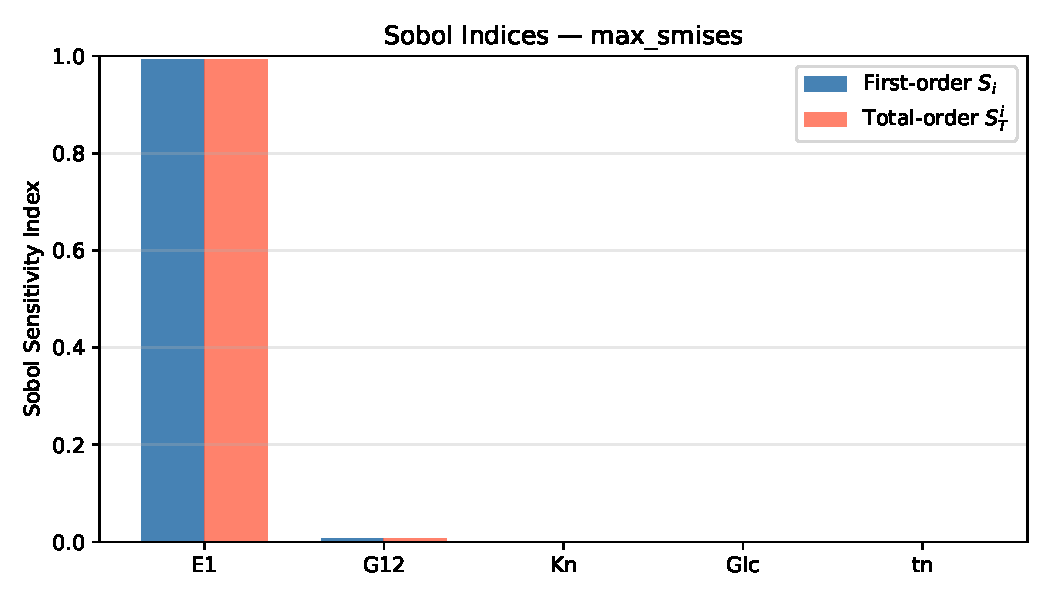
\includegraphics[width=0.8\textwidth]{figures/pce_uq/sobol_max_smises.pdf}
    \caption{Sobol sensitivity indices for max von Mises stress (degree~2). $E_1$ accounts for 99.2\% of output variance.}
    \label{fig:sobol_smises}
\end{figure}

\begin{figure}[h]
    \centering
    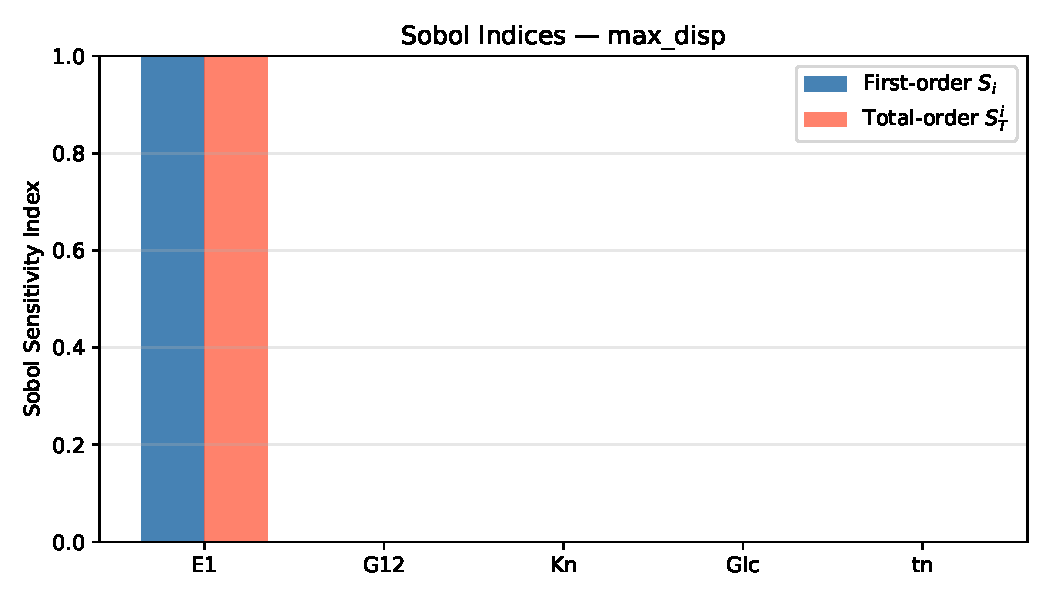
\includegraphics[width=0.8\textwidth]{figures/pce_uq/sobol_max_disp.pdf}
    \caption{Sobol sensitivity indices for max displacement (degree~2). $E_1$ dominates with $S_{E_1} = 0.9995$.}
    \label{fig:sobol_disp}
\end{figure}

\subsection{Surrogate Accuracy: PCE vs Neural Network}

\begin{table}[h]
\centering
\caption{Leave-one-out (LOO) RMSE comparison between PCE and NN surrogates.}
\begin{tabular}{lcccc}
\toprule
QoI & PCE deg=2 & PCE deg=3 & NN deg=2 data & NN deg=3 data \\
\midrule
$\sigma_\text{vM}^\text{max}$ (MPa) & $\mathbf{9.4\times10^{-4}}$ & $1.5\times10^{-3}$ & $7.2\times10^{-4}$ & $1.77\times10^{-2}$ \\
$d^\text{max}$                       & 0                          & 0                   & $\approx 0$        & $\approx 0$ \\
$u^\text{max}$ (mm)                  & $\mathbf{4.2\times10^{-5}}$ & $7.1\times10^{-5}$ & $2.7\times10^{-5}$ & $1.6\times10^{-3}$ \\
\bottomrule
\end{tabular}
\label{tab:rmse}
\end{table}

Three features of the comparison in Table~\ref{tab:rmse} are worth drawing out. The PCE expansion at degree~2 attains the lowest leave-one-out error of any configuration, and, tellingly, its degree-3 counterpart performs slightly \emph{worse}: fitting 56 coefficients to 286 points introduces estimation variance in the redundant high-order terms without any compensating reduction in bias, which is the classic symptom of mild over-parameterisation on an almost-linear response. The neural network exhibits the same pathology far more sharply --- its error degrades by an order of magnitude between the 66- and 286-point sets --- because a fixed architecture carrying several thousand weights cannot avoid overfitting when the underlying map is this smooth. In absolute terms, a PCE leave-one-out RMSE below $10^{-3}$~MPa against a nominal stress of $\approx 210$~MPa is a relative error of roughly $5\times10^{-4}\%$, so the surrogate error is entirely negligible beside the manufacturing-induced response scatter it is meant to characterise. The interpretability gap reinforces the same conclusion: the PCE returns the Sobol indices analytically from its coefficients, whereas the network would require a separate Monte Carlo sensitivity study to recover the same information.

%------------------------------------------------------------------
\section{Reliability Analysis}
%------------------------------------------------------------------

\subsection{Failure Probability Formulation}

The failure probability for an event $F = \{G(\xi) > b\}$ is:
\begin{equation}
    P_f = P(G(\xi) > b) = \int_F f_\xi(x)\,\mathrm{d}x
\end{equation}
where $f_\xi$ is the joint PDF of inputs and $b$ is the failure threshold. With $P_f$ estimated via Monte Carlo on the PCE surrogate:
\begin{equation}
    \hat{P}_f = \frac{1}{N}\sum_{i=1}^{N} \mathbf{1}_{F}(\xi^{(i)}), \quad \xi^{(i)} \sim f_\xi
\end{equation}

The reliability index $\beta$ is defined as $\beta = -\Phi^{-1}(P_f)$, where $\Phi$ is the standard normal CDF.

\subsection{Results}

With $\sigma_\text{vM}^\text{max}$ mean of 209.7~MPa and standard deviation of 2.38~MPa, the stress distribution is far from the 1{,}200~MPa threshold. Monte Carlo sampling of $10^6$ realisations on the PCE surrogate yields:
\begin{equation}
    P_f = P(\sigma_\text{vM}^\text{max} > 1200\ \text{MPa}) = 0 \qquad \Rightarrow \qquad \beta = \infty
\end{equation}

This result holds for both degree-2 and degree-3 PCE. Even a $6\sigma$ stress event ($209.7 + 6\times2.38 = 224$~MPa) remains well below failure.

The SDEG $= 0$ result confirms that the adhesive interface operates entirely within its elastic regime regardless of manufacturing variability, at the static design load level considered.

\begin{figure}[h]
    \centering
    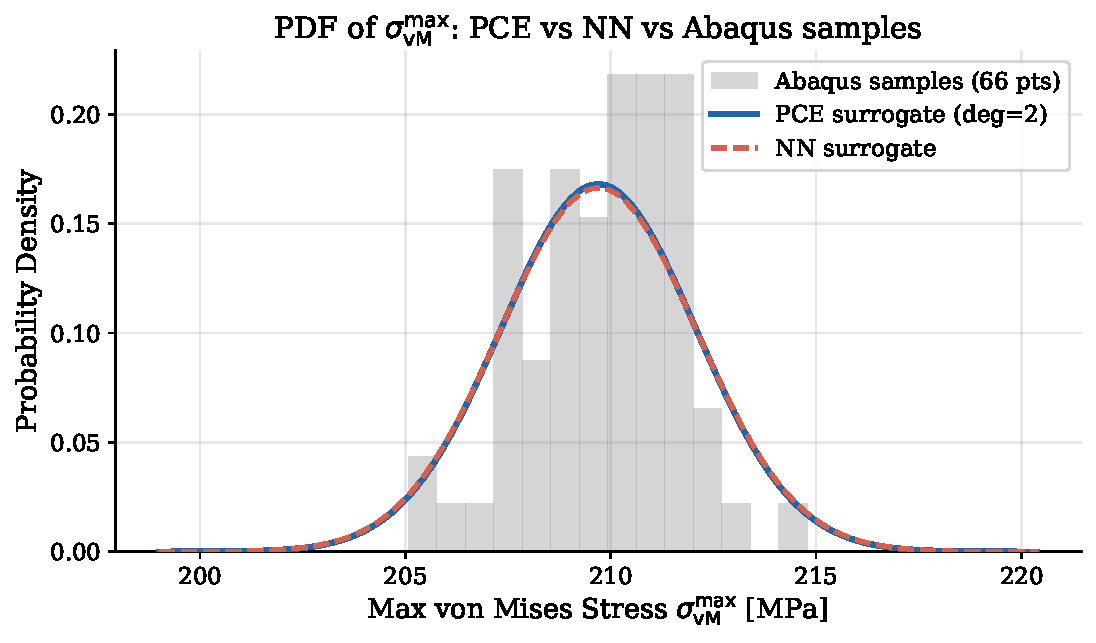
\includegraphics[width=0.8\textwidth]{figures/pce_uq/pdf_max_smises.pdf}
    \caption{PDF of max von Mises stress: PCE surrogate (blue), NN surrogate (orange), and Abaqus sample points (histogram). Both surrogates agree well. Degree~2.}
    \label{fig:pdf_smises}
\end{figure}

\begin{figure}[h]
    \centering
    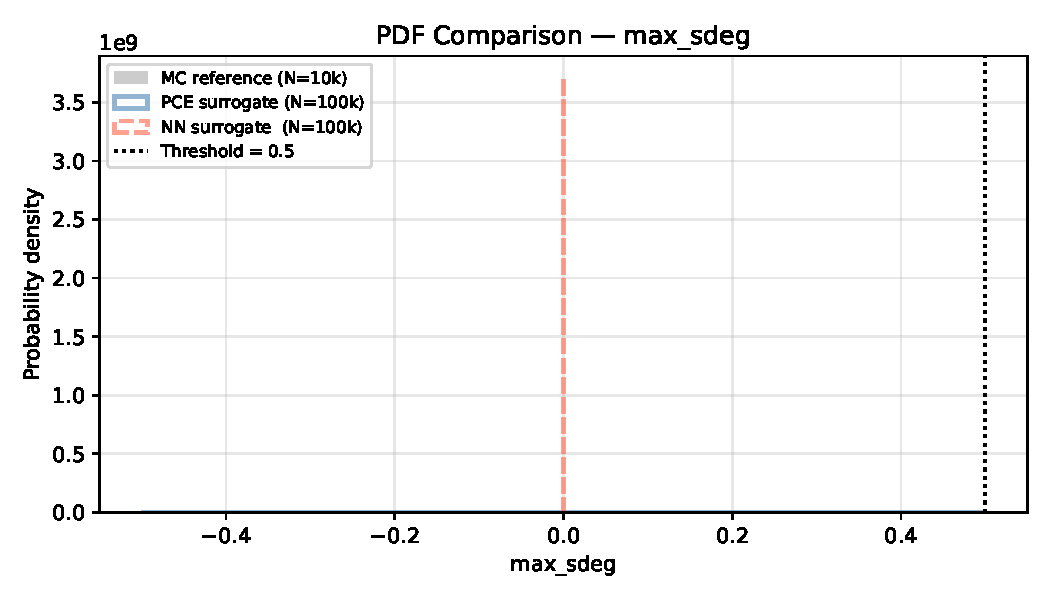
\includegraphics[width=0.8\textwidth]{figures/pce_uq/pdf_max_sdeg.pdf}
    \caption{PDF of max scalar damage variable (SDEG): all 66 Abaqus samples return SDEG $= 0$, confirming no cohesive damage initiation.}
    \label{fig:pdf_sdeg}
\end{figure}

\begin{figure}[h]
    \centering
    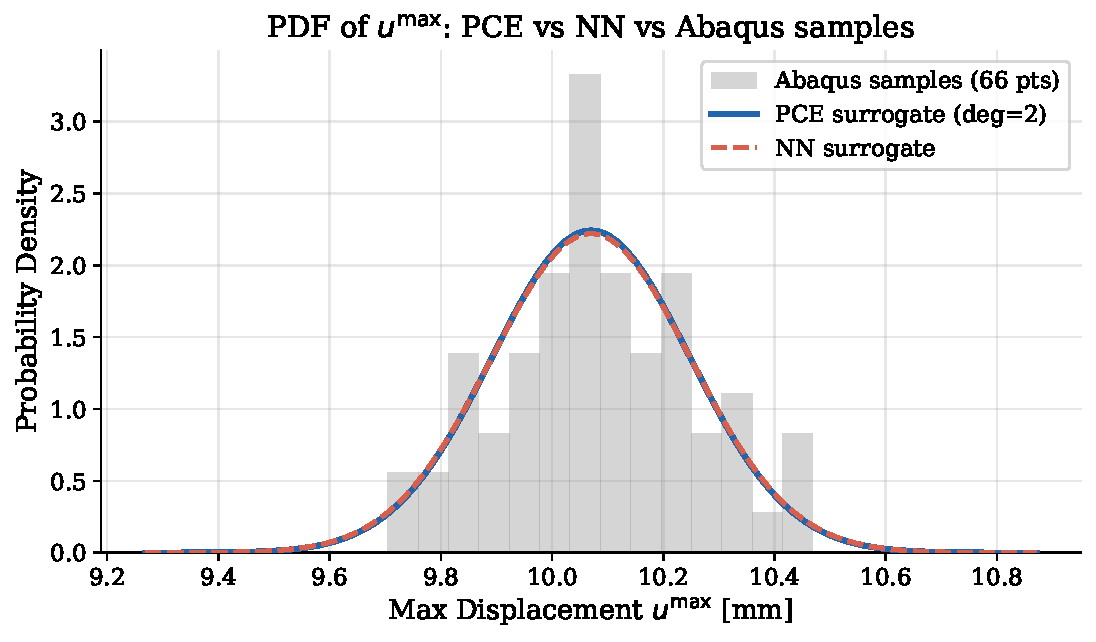
\includegraphics[width=0.8\textwidth]{figures/pce_uq/pdf_max_disp.pdf}
    \caption{PDF of max displacement: PCE vs NN surrogate comparison. Degree~2.}
    \label{fig:pdf_disp}
\end{figure}

\begin{figure}[h]
    \centering
    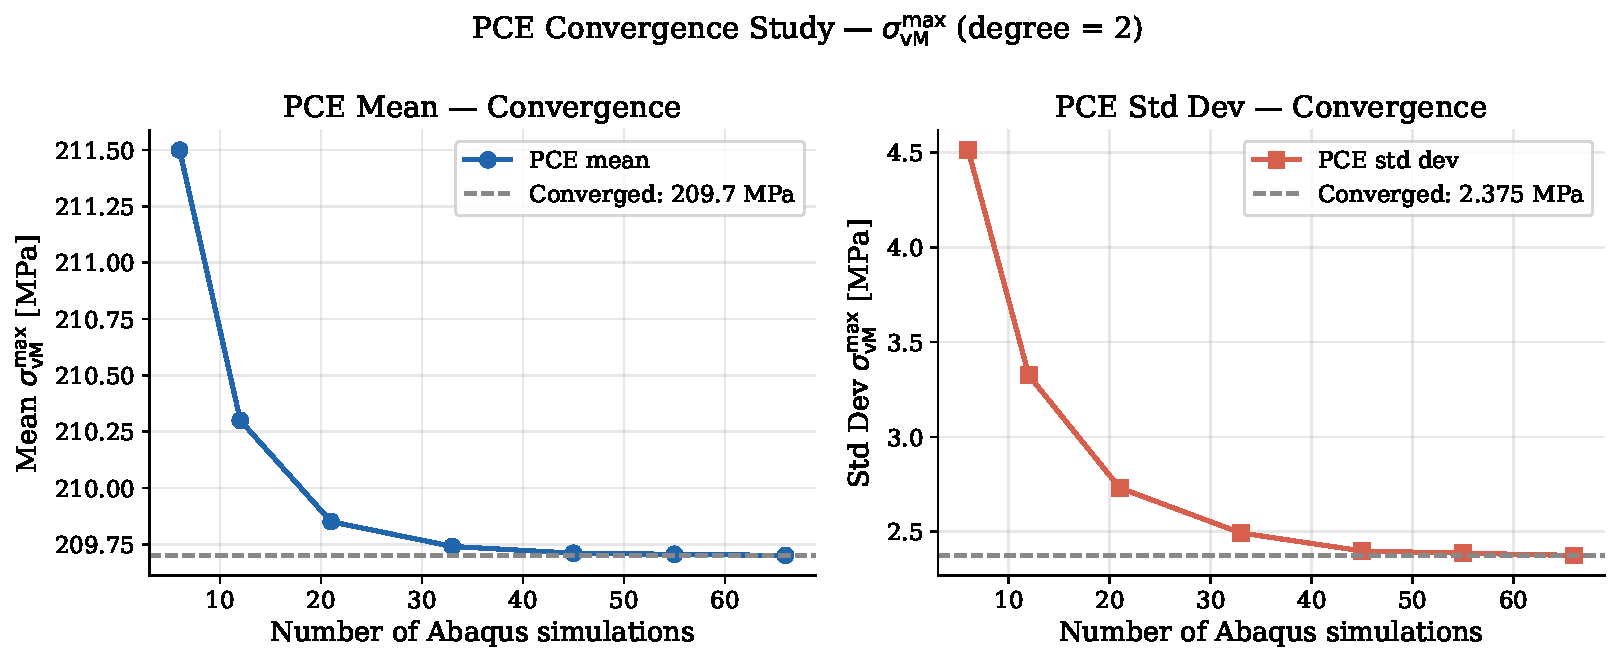
\includegraphics[width=\textwidth]{figures/pce_uq/convergence_max_smises.pdf}
    \caption{PCE convergence study for max von Mises stress (degree~2). Mean and standard deviation stabilise by 66 quadrature points.}
    \label{fig:conv_smises}
\end{figure}

\begin{figure}[h]
    \centering
    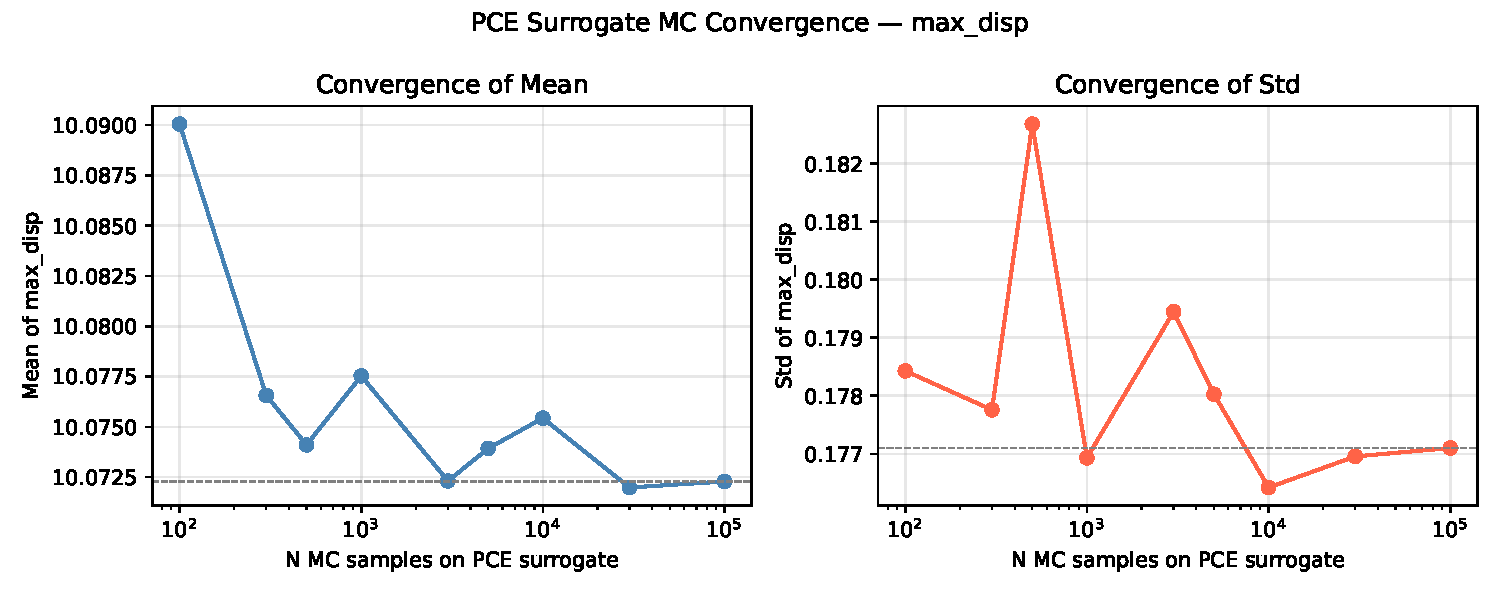
\includegraphics[width=\textwidth]{figures/pce_uq/convergence_max_disp.pdf}
    \caption{PCE convergence study for max displacement (degree~2). Both statistics are fully converged at 66 simulations.}
    \label{fig:conv_disp}
\end{figure}

%------------------------------------------------------------------
\section{Discussion}
%------------------------------------------------------------------

\subsection{Why Does $E_1$ Dominate?}
\label{sec:whye1}

The dominance of $E_1$ is best understood through a first-order propagation argument rather than treated as a numerical curiosity. For a response $Y$ that is smooth in the inputs, the output variance is approximated to first order by
\begin{equation}
    \mathrm{Var}(Y) \approx \sum_{i=1}^{d} \left( \frac{\partial Y}{\partial \xi_i} \right)^2 \sigma_{\xi_i}^2 ,
\end{equation}
so each parameter's contribution scales with the product of its local sensitivity \emph{and} its variance --- not with either quantity alone. The fairing panel carries the design pressure predominantly through in-plane membrane action, for which both the peak skin stress and the global deflection are set by the axial laminate stiffness $E_1 t$. The response is therefore close to linear in $E_1$, giving a large $\partial Y/\partial E_1$, while $E_1$ simultaneously carries a non-negligible 5\% manufacturing scatter; the product of the two places almost the entire output variance on this single parameter. The shear modulus $G_{12}$ is the instructive counter-example: although its 10\% CoV is twice that of $E_1$, the membrane-dominated kinematics make $\partial Y/\partial G_{12}$ small, so the larger input scatter is suppressed in the output and only $\sim 0.8\%$ of the stress variance survives. The sensitivity ranking is thus governed not by which parameter is most uncertain, but by which uncertainty the structure is mechanically configured to amplify --- a distinction that the raw Sobol numbers alone do not make explicit.

\subsection{Why Is SDEG Identically Zero?}
\label{sec:whysdeg}

That the cohesive interface remains undamaged across all 352 sampled configurations is a physical result with a clear load-margin explanation, but it also carries a methodological consequence that deserves to be stated plainly. The Step-2 load represents the static design-point pressure, comfortably within the elastic envelope of the adhesive: at nominal properties the interface traction stays below the cohesive strength $t_n$, and even at the $\pm 50\%$ truncation bounds on $K_n$, $t_n$ and $G_{Ic}$ the traction never reaches the damage-initiation criterion. Damage is therefore not merely improbable but absent from the entire sampled domain. The consequence is that the three cohesive parameters are \emph{structurally unidentifiable} in this study: because they never alter any QoI, no amount of additional sampling could assign them a non-zero Sobol index, and the nominally five-dimensional uncertainty problem collapses --- at this load level --- to an effectively one-dimensional problem in $E_1$. A study aimed at characterising the CZM parameters would have to raise the load into the damage-onset regime or introduce an explicit defect or impact scenario; under the present load, the most honest statement is that the data are simply uninformative about them.

\subsection{PCE vs Neural Network: Summary Comparison}

\begin{table}[h]
\centering
\caption{Qualitative comparison of PCE and NN surrogates for this problem.}
\begin{tabular}{lll}
\toprule
Criterion & PCE (this work) & NN surrogate \\
\midrule
Training data required & 66 points (deg=2)    & 66--286 points \\
Accuracy (LOO RMSE)    & $\sim 10^{-4}$        & $10^{-4}$ to $10^{-2}$ \\
Convergence with data  & Stable (deg=2 optimal) & Degrades (overfitting) \\
Sobol indices          & Analytical, exact      & Requires separate MC \\
Interpretability       & High                   & Low (black-box) \\
Applicable to          & Forward UQ, reliability & SHM, defect detection \\
\bottomrule
\end{tabular}
\label{tab:compare}
\end{table}

The contrast in Table~\ref{tab:compare} should not be read as a generic claim that polynomial chaos is ``better'' than a neural network, but as a statement about the match between method and problem. PCE encodes a strong prior --- that the response is a low-order polynomial in the inputs --- and when that prior is correct, as it is for this smooth, membrane-dominated response, it extracts accurate statistics from very few samples and returns the sensitivity information for free. The MLP encodes almost no prior and must learn the response shape from data; with only 66--286 samples and several thousand weights it sits in a heavily over-parameterised regime, which is precisely why its out-of-sample error \emph{grows} when the training set is enlarged from 66 to 286 points. The two surrogates therefore occupy different niches rather than competing on a single scale: PCE for forward uncertainty quantification and reliability on smooth, low-dimensional responses, and data-driven networks for the high-dimensional, strongly nonlinear, or field-valued problems --- defect detection and structural health monitoring among them --- where a polynomial prior would be too restrictive to be useful.

\subsection{Degree Convergence}

That the degree-2 (66-sample) and degree-3 (286-sample) statistics agree to four significant figures is more than a convergence check; it quantifies the curvature of the response surface. Had the QoIs depended appreciably on second- or higher-order terms, the additional 220 simulations of the degree-3 grid would have shifted the mean or, more sensitively, the standard deviation. Their failure to do so confirms that a quadratic basis already saturates the achievable accuracy. This reading is reinforced by the leave-one-out results of Table~\ref{tab:rmse}, where the degree-3 surrogate is marginally \emph{less} accurate than degree~2 --- a signature of variance from fitting redundant high-order coefficients rather than of bias from an inadequate basis. For this class of smooth, small-deformation structural response, degree~2 is therefore not a compromise but the appropriate model order.

\subsection{Limitations and Critical Reflection}
\label{sec:limits}

Several limitations qualify the conclusions above and define the regime in which they hold.

First, the reported failure probability of exactly zero should be read as ``below the resolution of the analysis'' rather than as a literal guarantee of safety. Monte Carlo sampling of $10^6$ surrogate realisations can only resolve probabilities down to $\mathcal{O}(10^{-6})$, and, more fundamentally, the surrogate is evaluated over truncated-normal inputs bounded at $\pm 50\%$ of nominal. Events in the far tail of the material distribution --- precisely those that dominate genuine structural risk --- lie outside both the sampled domain and the range over which the PCE was fitted, where it cannot be trusted to extrapolate. The defensible statement is therefore that, under the assumed input model and design load, the mean stress lies more than 400 standard deviations below the failure threshold --- $(1200-209.7)/2.38 \approx 416\sigma$ --- so the failure probability is negligible \emph{within the model's resolution}.

Second, the five inputs are treated as statistically independent, whereas the elastic constants of a CFRP ply share common physical drivers --- fiber volume fraction, cure quality --- and are in reality positively correlated. The proportional scaling applied to the dependent moduli imposes perfect correlation on those quantities while independence is assumed among the five primary variables, an internally inconsistent simplification. Because $E_1$ dominates so completely, the headline conclusions are robust to this assumption; however, a correlated input model would be required before the small $G_{12}$ contribution could be interpreted quantitatively.

Third, the study models a single representative panel rather than the complete fairing. Boundary conditions, shell curvature, and load introduction at the panel edges are idealised, so the absolute stress level (209.7~MPa) should be regarded as representative of the panel coupon rather than as a certified margin for the flight structure.

Fourth, only aleatory uncertainty in the material parameters is propagated. The epistemic error of the deterministic finite-element model itself --- mesh discretisation, the BK mixed-mode law, the linear-elastic honeycomb idealisation --- is not quantified and would add to the reported response variance in a complete uncertainty budget.

Finally, surrogate accuracy is assessed by leave-one-out cross-validation on the quadrature samples rather than against an independent validation set. For a response this smooth the distinction is minor, but for stiffer nonlinearities an out-of-sample test would be necessary to exclude optimistic error estimates.

None of these caveats overturns the central finding --- that fiber-direction modulus controls the structural variability and that the panel is comfortably reliable under the design load --- but each delimits the conditions under which it applies, and each points to a concrete extension: a correlated input model, a higher load level that activates the cohesive zone, and a full-fairing model with quantified discretisation error.

%------------------------------------------------------------------
\section{Conclusion}
%------------------------------------------------------------------

Non-intrusive Polynomial Chaos Expansion with Smolyak sparse quadrature was applied to quantify how manufacturing variability propagates through an Abaqus/Standard model of the JAXA H3 CFRP/aluminum-honeycomb fairing panel. The study shows that a second-order expansion built from only 66 simulations already captures the full response statistics: a third-order expansion costing 286 simulations reproduces the mean and standard deviation to four significant figures and is, if anything, marginally less accurate out-of-sample. Degree~2 is thus identified as the correct model order for this smooth, near-linear response rather than as an economy measure --- a distinction that matters when defending the result, because it rests on the demonstrated curvature of the response surface, not merely on a cost trade-off.

The sensitivity analysis yields a single, actionable message for manufacturing. The fiber-direction modulus $E_1$ governs more than 99\% of the variance in both peak stress and deflection, so tightening the quality control of $E_1$ --- through fiber-volume-fraction and cure consistency --- is by far the most effective lever for reducing structural variability, whereas tolerances on shear stiffness and on the adhesive parameters are, at this load level, of little consequence. Under the design pressure the panel is reliable by a wide margin, with a peak von Mises stress of 209.7~MPa at only 17.5\% of the CFRP strength and a stress coefficient of variation of 1.13\%, and with the cohesive interface never leaving its elastic regime.

For this smooth, low-dimensional, and near-linear problem the PCE surrogate is preferable to the neural-network alternative on every axis that matters here --- data economy, accuracy, and the analytical availability of Sobol indices --- although that balance would shift towards data-driven surrogates for higher-dimensional or strongly nonlinear responses such as post-damage behaviour. The principal limitation of the present work is that the cohesive parameters remain unidentifiable because the design load never initiates damage; the natural continuation is therefore to repeat the analysis at a load level that activates the cohesive zone, under a correlated input model and a full-fairing geometry, so that the reliability of the bonded interface --- and not only of the skin --- can be assessed.

%------------------------------------------------------------------
\bibliographystyle{unsrt}
\begin{thebibliography}{9}

\bibitem{ghanem1991}
R.~G.~Ghanem and P.~D.~Spanos,
\textit{Stochastic Finite Elements: A Spectral Approach}.
Springer, 1991.

\bibitem{sudret2000}
B.~Sudret and A.~Der~Kiureghian,
``Stochastic Finite Element Methods and Reliability: A State-of-the-Art Report,''
Report No.\ UCB/SEMM-2000/08, University of California, Berkeley, 2000.

\bibitem{sudret2008}
B.~Sudret,
``Global sensitivity analysis using polynomial chaos expansions,''
\textit{Reliability Engineering \& System Safety}, vol.~93, no.~7, pp.~964--979, 2008.

\bibitem{smolyak1963}
S.~A.~Smolyak,
``Quadrature and interpolation formulas for tensor products of certain classes of functions,''
\textit{Dokl. Akad. Nauk SSSR}, vol.~148, no.~5, pp.~1042--1045, 1963.

\bibitem{fajraoui2017}
N.~Fajraoui, S.~Marelli, and B.~Sudret,
``Sequential design of experiment for sparse polynomial chaos expansions,''
\textit{SIAM/ASA J. Uncertainty Quantification}, vol.~5, no.~1, pp.~1061--1085, 2017.

\bibitem{saltelli2008}
A.~Saltelli et al.,
\textit{Global Sensitivity Analysis: The Primer}.
Wiley, 2008.

\bibitem{faber2012}
M.~H.~Faber,
\textit{Statistics and Probability Theory}.
Springer, 2012.

\end{thebibliography}

%------------------------------------------------------------------
\appendix
\section{Software and Computational Environment}

\begin{table}[h]
\centering
\caption{Software versions and computational environment.}
\begin{tabular}{ll}
\toprule
Component & Version / Details \\
\midrule
Abaqus/Standard & 2024 \\
Python          & 3.12 \\
chaospy         & latest \\
PyTorch         & 2.10.0 \\
Server          & 172.17.36.98, 4$\times$GPU \\
Total CPU-hours & 352 jobs $\times$ $\approx$4~min $\approx$ 23~h \\
\bottomrule
\end{tabular}
\label{tab:env}
\end{table}

\section{Repository File Structure}

\begin{verbatim}
Stochastic-Finite-Element-Methods-2026/
  pce_driver.py              # PCE UQ main driver (Smolyak, chaospy)
  extract_pce_qoi.py         # Abaqus Python QoI extractor (odbAccess)
  reliability_analysis.py    # Post-processing, Sobol indices, plots
  report.pdf / slides.pdf    # Report and presentation
  figures/
    pce_uq/                  # Plots for degree=2 (66 jobs)
    pce_uq_deg3/             # Plots for degree=3 (286 jobs)
\end{verbatim}

Abaqus ODB files ($\approx 293$~MB each) are stored on the LUH compute server and not included in the repository.

\end{document}
